\section{Theorie}

\subsection{Berechnung der Suszeptibilität paramagnetischer Substanzen}

\begin{align}
    \intertext{Die magnetische Flussdichte $\vec{\text{B}}$ setzt sich aus der magnetischen Feldstärke $\vec{\text{H}}$, der Induktionskonstante $\mu_{0}$ und der Magnetisierung $\vec{\text{M}}$ im Vakuum zusammen}
    \vec{\text{B}} = \mu_{0} \vec{\text{H}} + \vec{\text{M}}\,. \notag
    \intertext{Durch die Abhängigkeit der Magnetisierung von der magnetischen Feldstärke folgt der Ausdruck}
    \vec{\text{M}} = \mu_{0}\, \chi\, \vec{\text{H}}\,. \label{1}
    \intertext{Der Faktor $\chi$ ist hierbei die Suszeptibilität, welche Temperatur T und $\vec{\text{H}}$ anhängig ist.
    Der Paramagnetismus in diesem Versuch ist nicht in jedem Material zu beobachten, nur bei Stoffen deren Drehimpuls nicht verschwindet. 
    Das liegt an der Orientierung der magnetischen Momente, welche mit dem Drehimpuls gekoppelt sind, die in einem außen anliegendem Feld erzeugt werden. 
    Die Ausrichtung ist jedoch eine thermische Bewegung der Atome, wodurch der Paramagnetismus temperaturabhängig ist und die Orientierung dadurch dauerhaft verändert.
    Dadurch das die Magnetischen Momente mit dem Drehimpuls gekoppelt sind wird diese Beziehung näher betrachtet.
    Der Gesamtdrehimpuls $\vec{\text{J}}$ setzt sich aus der Eigendrehung der Elektronen $\vec{\text{S}}$, dem Bahnimpuls $\vec{\text{L}}$ und dem Kerndrehimpuls zusammen.
    Der Kerndrehimpuls wird für den Paramagnetismus jedoch vernachlässigt}
    \vec{\text{J}} = \vec{\text{L}} + \vec{\text{S}}\,. \notag
    \intertext{Dabei sind die Drehimpulse $\vec{\text{L}}$ und $\vec{\text{J}}$ Summen aller Einzeldrehimpulse der Elektronen.
    Aus der Quantenmechanik folgt:}
    \vec{\mu}_{\text{L}} = - \frac{\mu_{\text{B}}}{\hbar}\, \vec{\text{L}} \label{2}\\
    \vec{\mu}_{\text{S}} = - \text{g}_{\text{S}}\frac{\mu_{\text{B}}}{\hbar}\,\vec{\text{S}}\,,\label{3}
    \intertext{mit dem Bohrschen Magneton $\mu_{\text{B}}$, und dem gyromagnetischen Verhältnis $\text{g}_{\text{S}}$.
    Bei Betrachtung der der Beträge hilft die Beziehung $\lvert \vec{\text{J}} \rvert = \sqrt{\text{J}(\text{J}+1)}\,\hbar$, welche für den Gesamtbahndrehimpuls und Gesamtspin analog ist.
    Daraus folgt: }
    \lvert \mu_{\text{L}} \rvert = \mu_{\text{B}} \sqrt{\text{L}(\text{L}+1)}\label{4} \\
    \lvert \mu_{\text{S}} \rvert = \text{g}_{\text{S}} \mu_{\text{B}} \sqrt{\text{S}(\text{S}+1)}\,.\label{5}
\end{align}

\begin{figure}[H] 
    \centering
    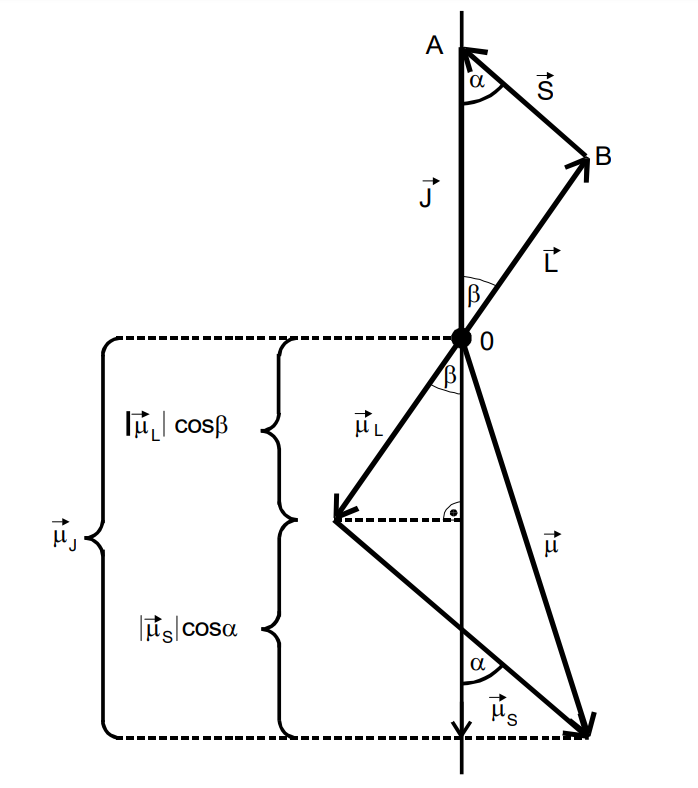
\includegraphics[height=70mm]{bilder/Ab1.png}
    \caption{Vektordiagramm aus den Drehimpulsvektoren einer Elektronenhülle und den daraus resultierenden magnetischen Momenten \cite{a1}.\label{Abbildung1} }
\end{figure}

\begin{align}
    \intertext{Durch die Abbildung \ref{Abbildung1} folgt die Beziehung}
    \lvert \vec{\mu}_{\text{J}} \rvert = \lvert \vec{\mu}_{\text{S}} \rvert \cos(\alpha) + \lvert \vec{\mu}_{\text{L}} \rvert \cos(\beta)\,. \notag
    \intertext{Durch die vereinfachte Annahme, dass $\text{g}_{\text{S}}$ den Wert zwei besitzt, folgt für $\lvert \vec{\mu}_{\text{J}} \rvert$}
    \lvert \vec{\mu}_{\text{J}} \rvert \approx \mu_{\text{B}} \sqrt{\text{J}(\text{J}+1)}\, \frac{3\text{J}(\text{J}+1) + (\text{S}(\text{S}+1) -  \text{L}(\text{L}+1))}{2\text{J}(\text{J}+1)}\label{6}
    \intertext{wobei der Bruchausdruck, der Landé-Faktor ist}
    \text{g}_{\text{J}}= \frac{3\text{J}(\text{J}+1) + (\text{S}(\text{S}+1) -  \text{L}(\text{L}+1))}{2\text{J}(\text{J}+1)}\label{7}
    \intertext{Die Richtungsquantelung ist ein weiterer Effekt der Quantenphysik, welcher besagt, dass der Winkel zwischen Lage von $ \lvert \vec{\mu}_{\text{J}} \rvert$ und dem außen angelegtem Feld nicht beliebig ist.
    Für die Z-Komponente ergibt sich}
    \mu_{\text{J}_{\text{z}}} = - \mu_{\text{B}} \text{g}_{\text{J}}\text{m}\, \label{8}
    \intertext{wobei m die Orientierungsquantenzah ist und der Winkel nur $2\text{J}+1$ verschiedene Einstellungen haben kann.
    Jede Einstellung hat ein eigene potentielle Energie mit der die Magnetisierung $\vec{M}$ bestimmt werden kann}
    \text{E} = - \vec{\mu}_{\text{J}} \cdot \vec{B} = \mu_{\text{J}_{\text{z}}\text{B}} = \mu_{\text{B}} \text{g}_{\text{J}} \text{m}\text{B}. \notag 
    \intertext{Dafür wird die Häufigkeit der auftretenden Winkel berechnet und mit der Formel (\ref{8}) multipliziert, sowie über alle möglichen Einstellungen summiert, wodurch sich nach Umformungen die Suszeptibilität $\chi$ ergibt}
    \chi = \frac{\mu_{0}\mu^{2}_{\text{B}}\text{g}^{2}_{\text{J}} \text{N} \text{J} (\text{J}+1)}{3\text{kT}}\,.\label{9}
    \intertext{N steht dabei für die Anzahl der Momente pro Volumeneinheit, k für die Boltzmann-Konstante und T für die Temperatur.
    Wenn die Temperatur hinreichend hoch ist gilt}
    \chi \approx \frac{1}{T}, \notag
    \intertext{was bekannt als das Curiesche Gesetz des Paramagnetismus ist.}
    \intertext{Ionen Seltener Erden haben einen starken Paramagnetismus, welcher zurückzuführen ist auf die Elektronen die in der vierten f-Schale der Elektronenhülle vorhanden sind.
    Der Drehimpuls, der durch die Anordnung der Elektronen innerhalb der Schale gegeben ist, wird durch die Hundschen Regeln beschrieben.} \notag
\end{align}

\begin{itemize}
    \item Das summieren der Spins $\vec{\text{s}}_{\text{i}}$ führt nach dem Pauli-Prinzip zum maximalen Gesamtspin $\vec{S} = \sum \vec{\text{s}}_{\text{i}}$
    \item Der Gesamtdrehimpuls ist gegeben durch $\vec{J} = \vec{L} - \vec{S}$ für eine weniger als halbgefüllte Schale und durch $\vec{J} = \vec{L} + \vec{S}$ für eine mehr als halbgefüllte Schale.
    \item Der maximale Drehimpuls setzt sich aus der Summierung aller Bahndrehimpulse zusammen, welche unter Beachtung der ersten Regel und dem Pauli-Prinzip gebildet werden können.
\end{itemize}

\subsection{Messverfahren zur Bestimmung der Suszeptibilität}

\begin{align}
    \intertext{Um die Suszeptibilität $\chi$ experimentell zu bestimmen wird eine Wheatstonsche Brücke, wie in Abbildung \ref{Abbildung2} gezeigt, verwendet.
    Wie im Schaltbild zu sehen sind zwei Spulen verbaut, welche möglichst die selbe Induktivität haben sollten.
    Die Suszeptibilität wird nämlich über die Induktivitätsdifferenz $\increment \text{L}$ zwischen der materiegefüllten Spule und der Luftspule bestimmt.
    Eine Methode die zum Bestimmen der Suszeptibilität sieht wie folgt aus.
    Zuerst wird die Brückenspannung $\text{U}_{\text{Br}}$ gemessen und abgeglichen, dadurch verschwindet die Brückenspannung.
    Als nächstes wird nun eine Spule mit Materie gefüllt und der daraus resultierenden Anstieg der Brückenspannung gemessen, wodurch die Suszeptibilität bestimmt werden kann.
    Bei Frequenzen die hinreichend hoch sind, also $\omega^2 \text{L}^2 \gg \text{R}^2$ gilt, kann durch Vereinfachungen sowie Umformungen die Suszeptibilität bestimmt werden durch}
    \chi (\omega \to \infty) = 4\frac{\text{F}}{\text{Q}} \frac{\text{U}_{\text{Br}}}{\text{U}_{\text{Sp}}}.\label{10}
    \intertext{Dabei stehen F für den Spulenquerschnitt und Q für den Querschnitt der Probe und $\text{U}_{\text{Sp}}$ für die Speisespannung.
    Die andere Methode besteht aus dem selben Verfahren wie bei der erste Methode, jedoch wird nach dem füllen einer Spule die Brückenspannung erneut abgeglichen und durch die Änderung der Abgleichelemente die Suszeptibilität bestimmt.
    Berechnen lässt sich diese, durch}
    \chi = 2 \frac{\increment \text{R}}{\text{R}_{3}}\frac{\text{F}}{\text{Q}}\,.\label{11}
    \intertext{ $\increment \text{R}$ steht dabei für die Differenz der Einstellungen am Potentiometer und $\text{R}_{3}$ für den ersten abgeglichenen Widerstand. } \notag
\end{align}

\begin{figure}[H] 
    \centering
    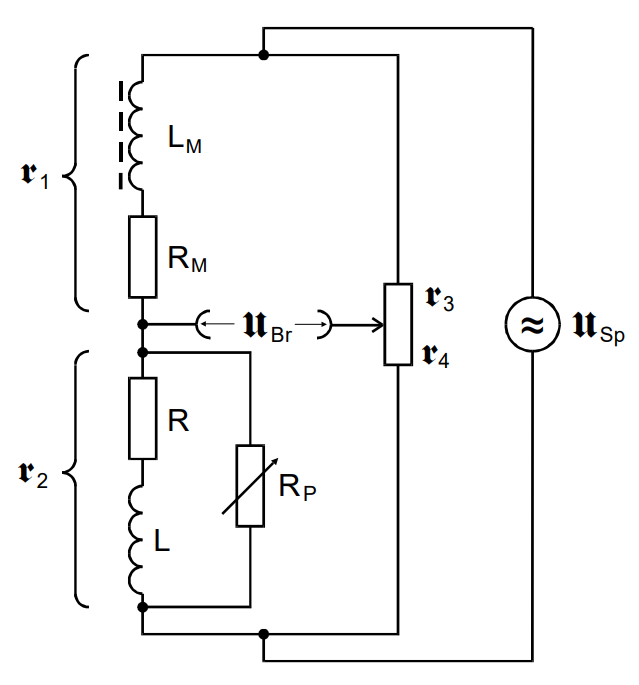
\includegraphics[height=80mm]{bilder/schaltung.png}
    \caption{Brückenschaltung für die Messung der Suszeptibilität \cite{a1}. \label{Abbildung2} }
\end{figure}

\subsection{Unterdrückung von Störspannungen bei der Messung kleiner Signalspannungen}

\begin{align*}
    \intertext{Bei Brückenschaltungen sind immer Störspannungen an den Ausgängen vorhanden. 
    Durch diese wird die Brückenspannung komplett überdeckt und die Messung der Suszeptibilität nicht möglich.
    Dies wird durch einen Selektivverstärker jedoch möglich, da bei dieser Messung monofrequente Signalspannung vorliegen und durch ein elektronischen Filter, wie der Selektivverstärker, nur bestimmte Spannungen mit bestimmten Frequenzen durchgelassen werden.
    Die Filterkurve von dem Selektivverstärker steht im Verhältnis von Ausgangsspannung $\text{U}_{\text{A}}$ zur Eingangsspannung $\text{U}_{\text{E}}$, ist abhängig von der Frequenz und wird in Abbildung \ref{Abbildung3} verbildlicht. }
\end{align*}

\begin{figure}[H] 
    \centering
    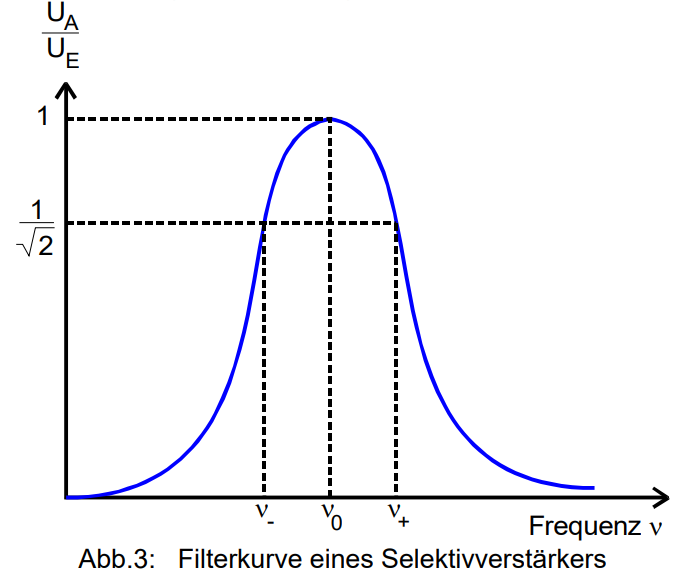
\includegraphics[height=70mm]{bilder/Ab3.png}
    \caption{Glockenkurve des Selektivverstärkers \cite{a1}. \label{Abbildung3} }
\end{figure}

\begin{align}
    \intertext{Die Breite dieser Kurve steht als Maß für die Wirksamkeit der Störspannungsunterdrückung, welcher im engen Zusammenhang mit der Güte Q steht}
    \text{Q} = \frac{\nu_{0}}{\nu_{+} - \nu_{-}}. \label{12}
    \intertext{Die Differenz der beiden Frequenzen wird bei dem Verhältnis $\frac{\text{U}_{\text{A}}}{\text{U}_{\text{E}}}$ an der Stelle $\frac{1}{\sqrt{2}}$ bestimmt. } \notag
\end{align}